\documentclass{article}

\usepackage{graphicx}

\title{Resume Database 2}
\author{Gany berdu sura }

\begin{document}

\maketitle{email : Ganysura29@gmail.com dan   password : ganyberdusura}

\section{Buka aplikasi oracle pada link https://apex.oracle.com/en/, kemudian sign in dengan email serta sandi yang telah terdaftar}
\begin{center}
    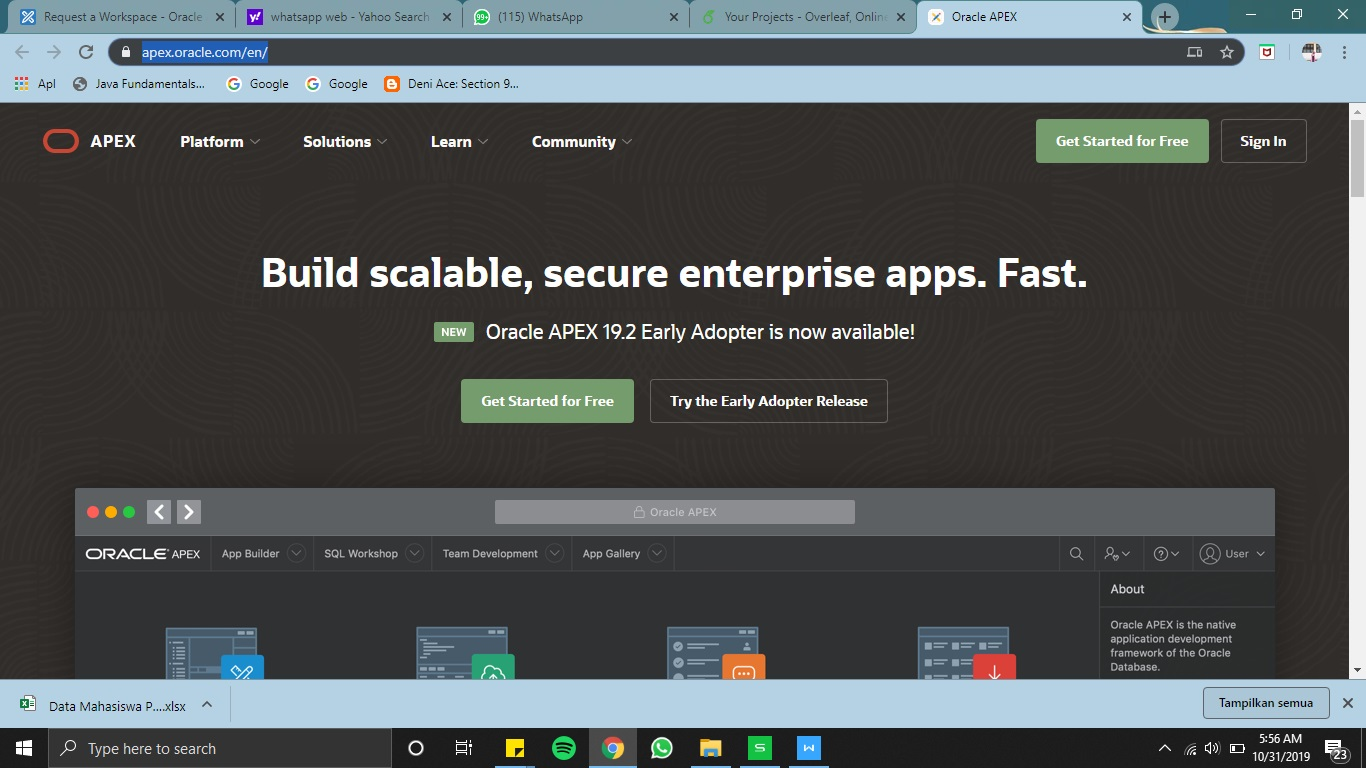
\includegraphics[width=.6\textwidth]{gambar/satu.jpg}
\end{center}
\section{Akan muncul tampilan seperti ini, masukan sandi, workspace serta sandi}
\begin{center}
    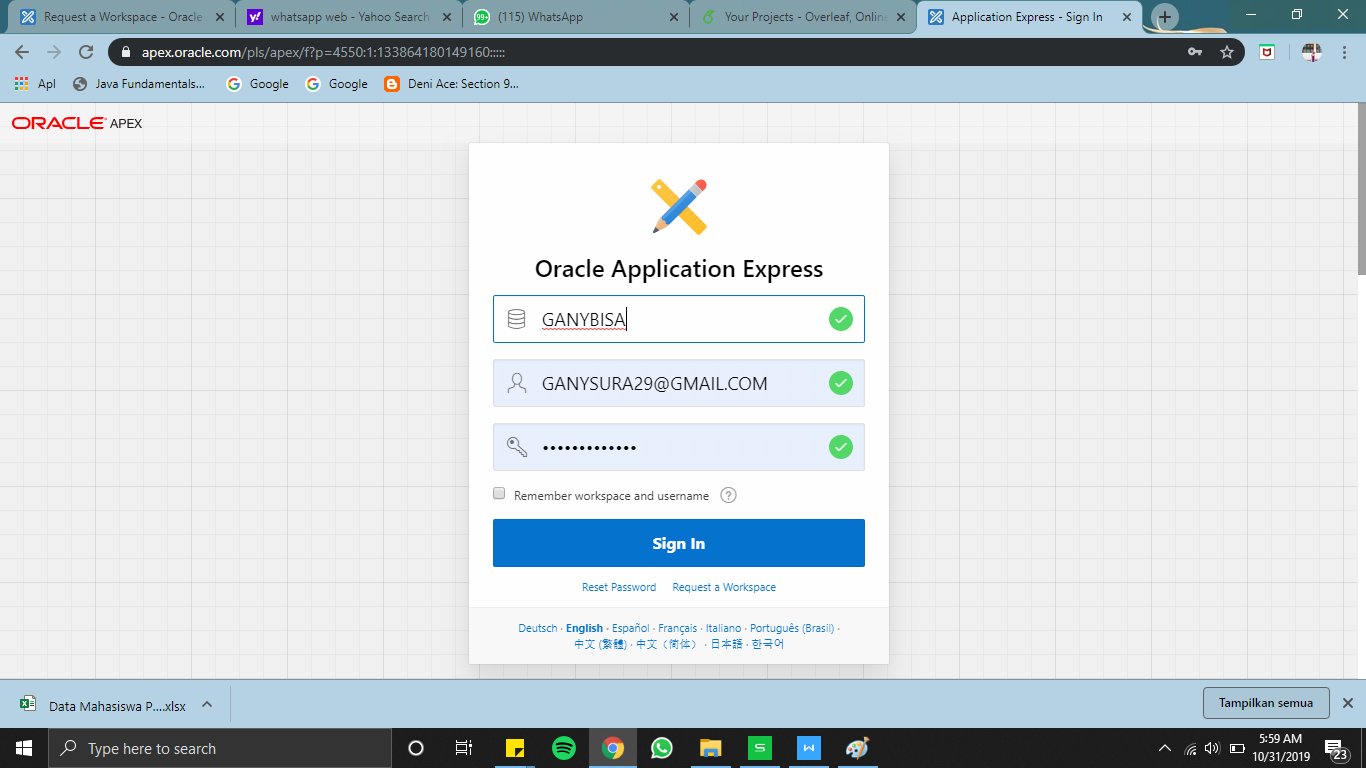
\includegraphics[width=.6\textwidth]{gambar/dua.png}
\end{center}
\section{Setelah masuk pilih apps buillder untuk membuat apps yang baru}
\begin{center}
    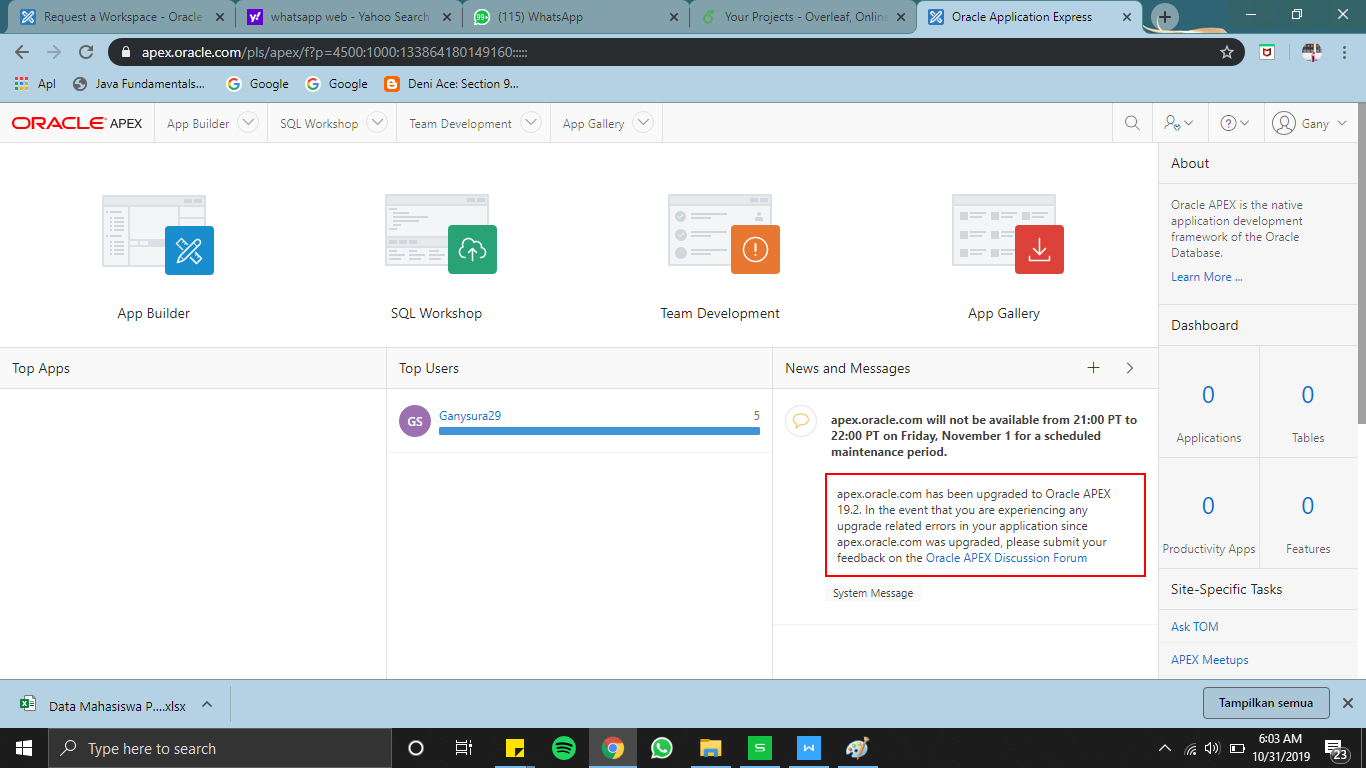
\includegraphics[width=.6\textwidth]{gambar/tiga.png}
\end{center}
\section{Kemudia pilih create, mengapa pilih import agar kita bisa memasukan file (.xlxs) atau dalam bentuk Exel yang telah kita buat.}
\begin{center}
    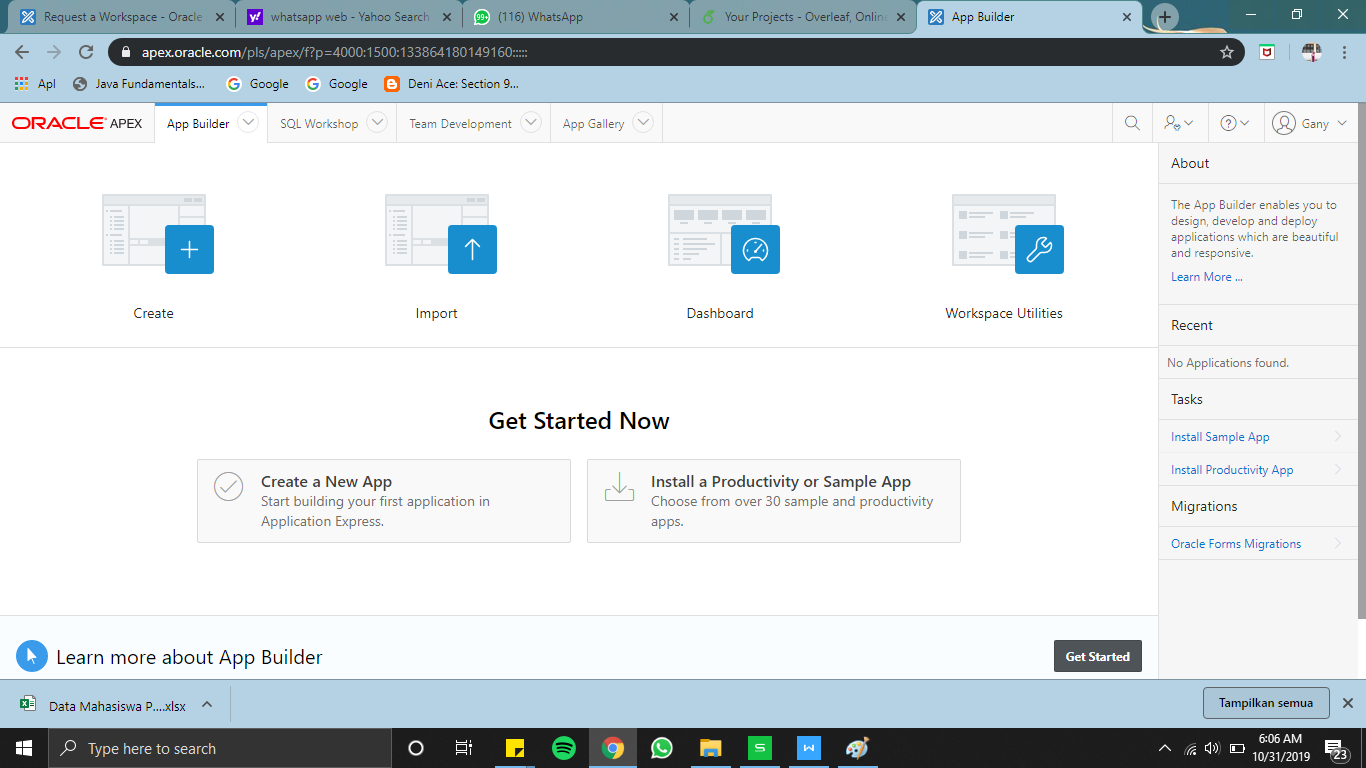
\includegraphics[width=.6\textwidth]{gambar/empat.png}
\end{center}
\section{Kemudian pilih from a file agara bisa mengambil data yang telah kita buat}
\begin{center}
    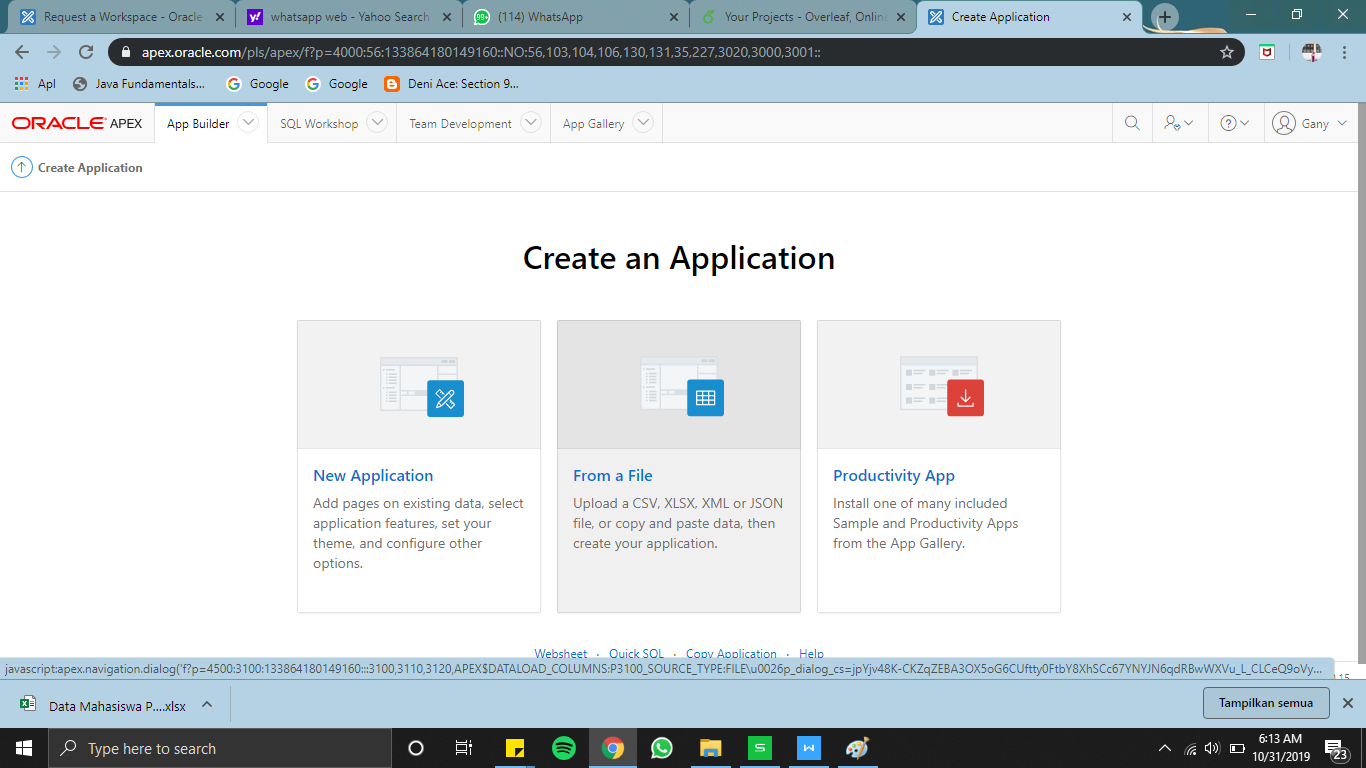
\includegraphics[width=.3\textwidth]{gambar/lima.png}
    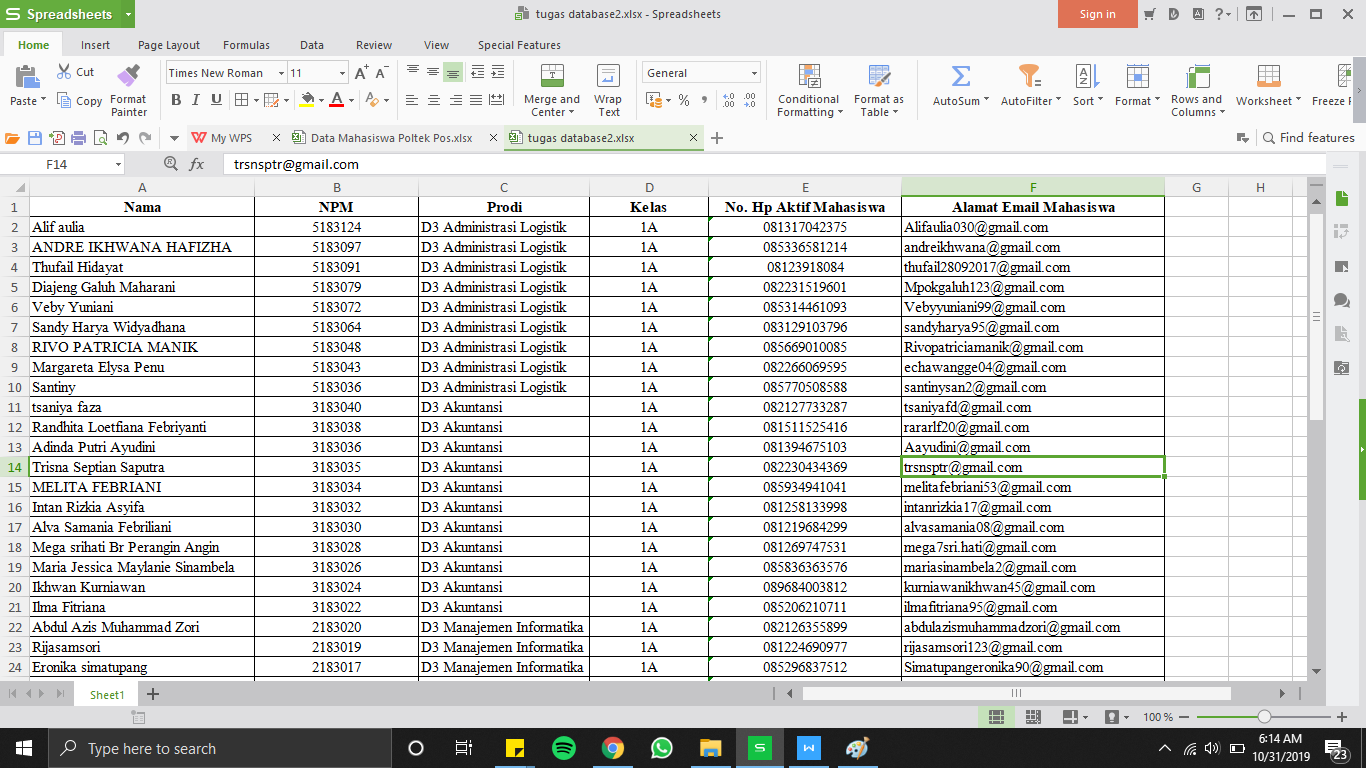
\includegraphics[width=.3\textwidth]{gambar/data exel.png}
\end{center}
\section{Drag file exel diatas kedalam text box tersebut, setelah data didrag dan filenya telah masuk rubah nama tabel yang akan dimasukin ke oracle apex, kemudian load data dan creat aplication}
\begin{center}
    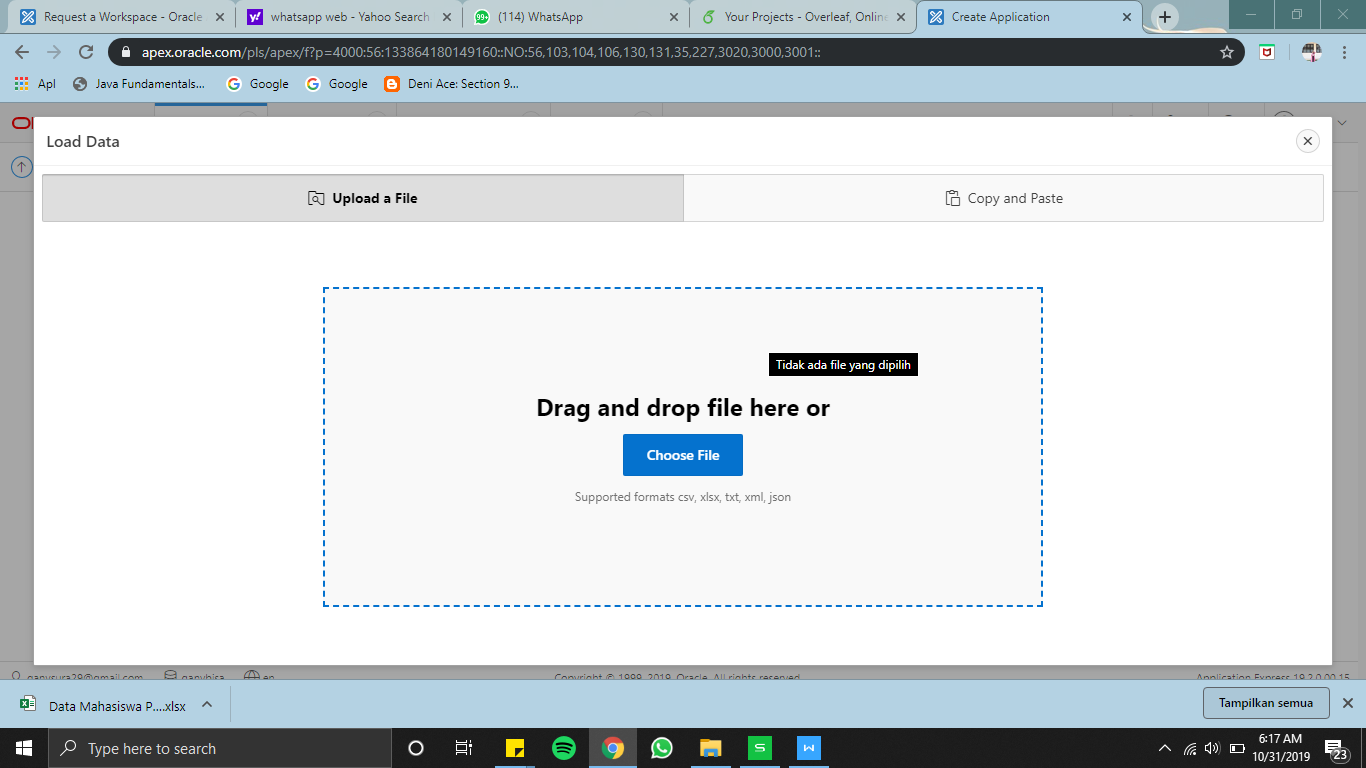
\includegraphics[width=.3\textwidth]{gambar/enam.png}
    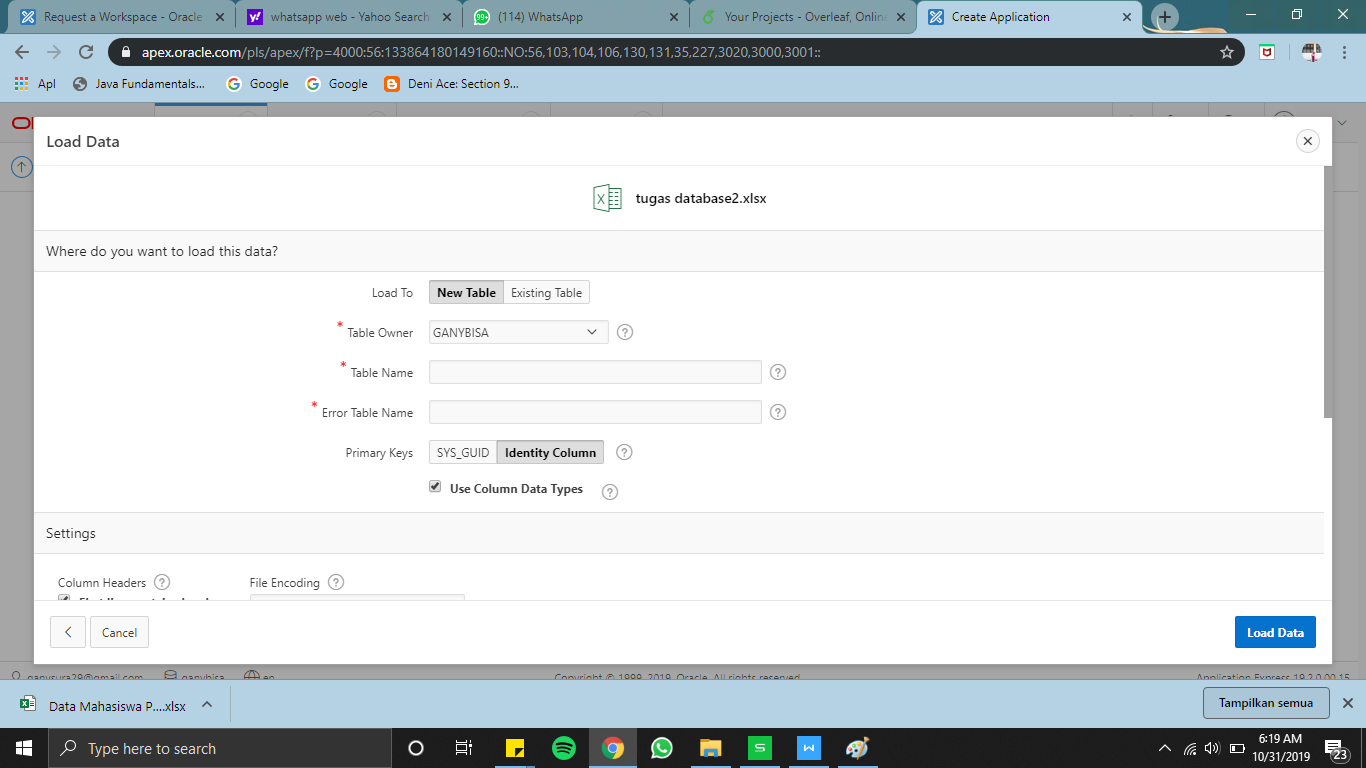
\includegraphics[width=.3\textwidth]{gambar/tujuh.png}
\end{center}
\section{Setelah succes jangan lupa mencentang semua kolom seperti dibawah ini kemudian create application kemudian di run application.
}
\begin{center}
    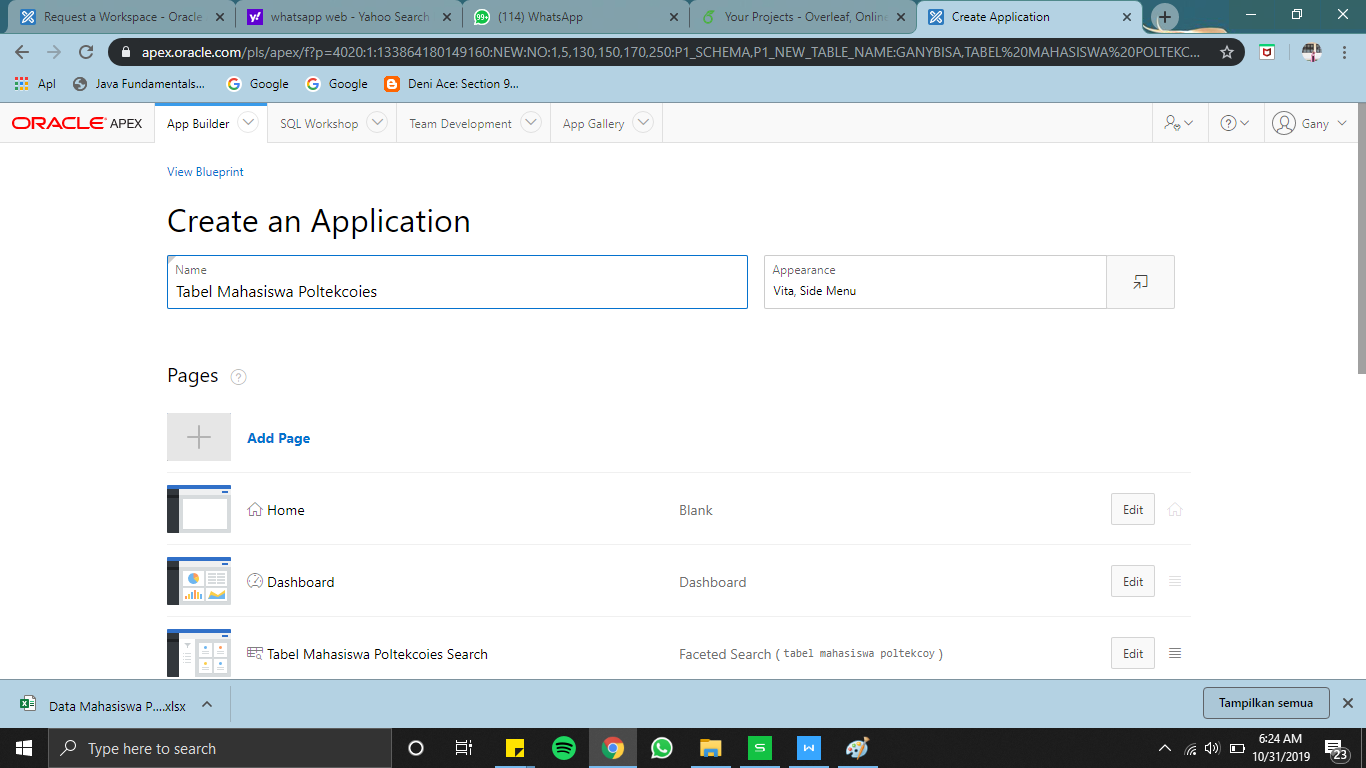
\includegraphics[width=.6\textwidth]{gambar/delapan.png}
    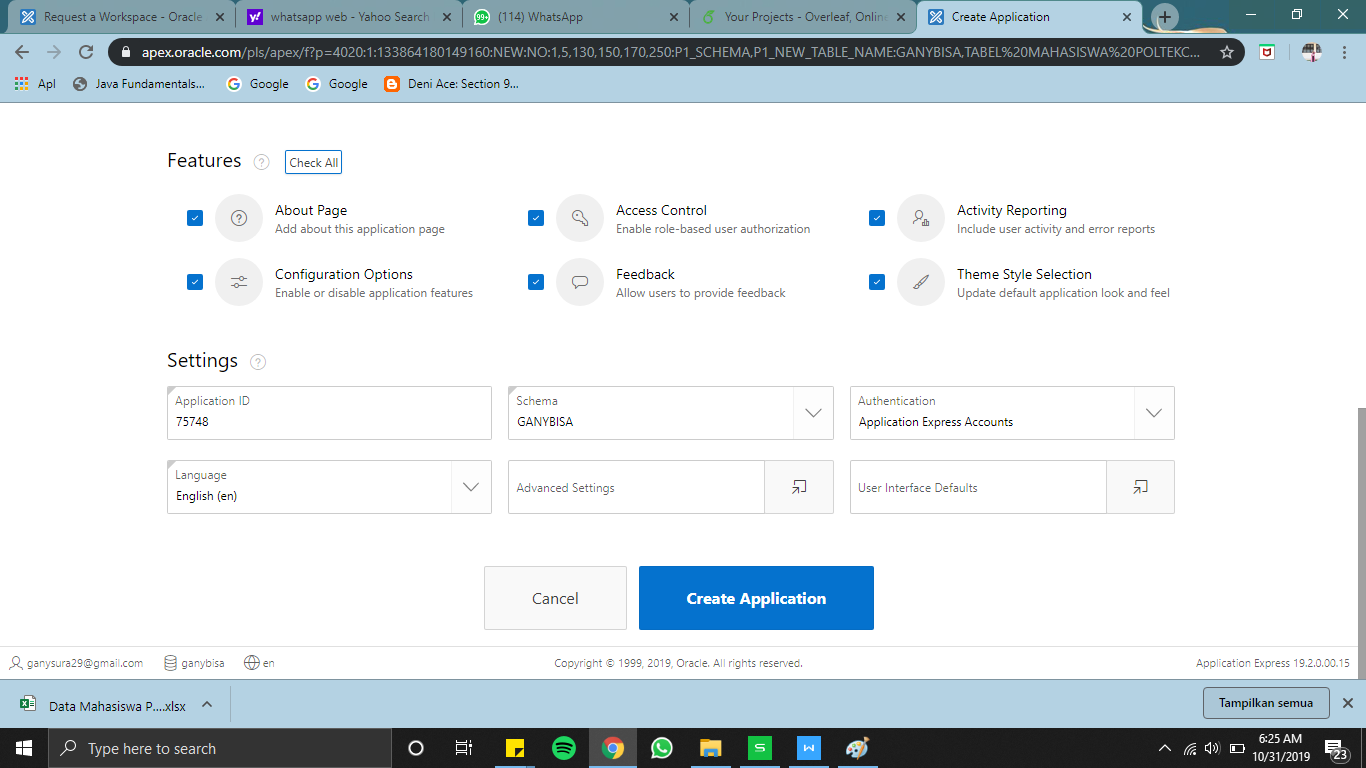
\includegraphics[width=.6\textwidth]{gambar/sembilan.png}
\end{center}
\section{Kemudian register lagi pake email dan password dan akan tampil tabel yang telah di buat pada exel tadi yang kemudian di extract ke oracle apec.}

\begin{center}
    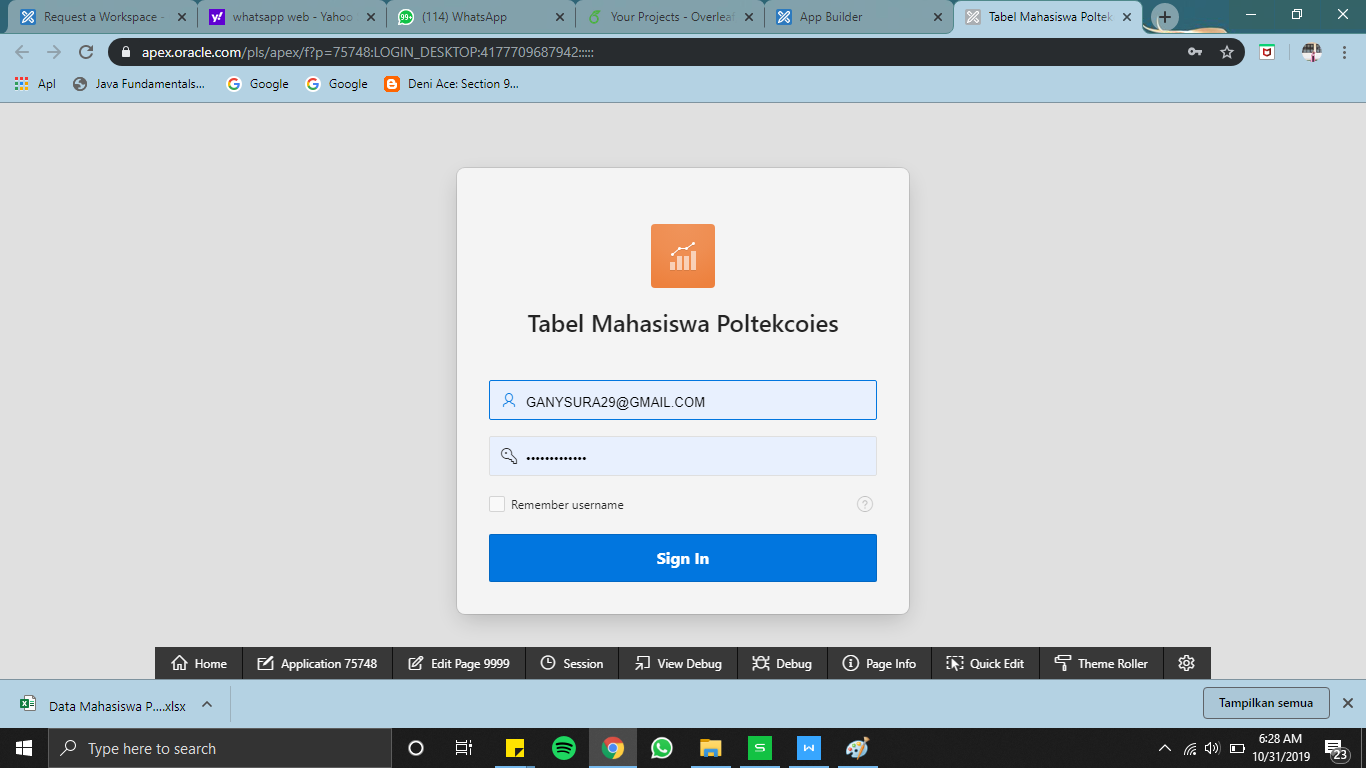
\includegraphics[width=.6\textwidth]{gambar/sepuluh.png}
    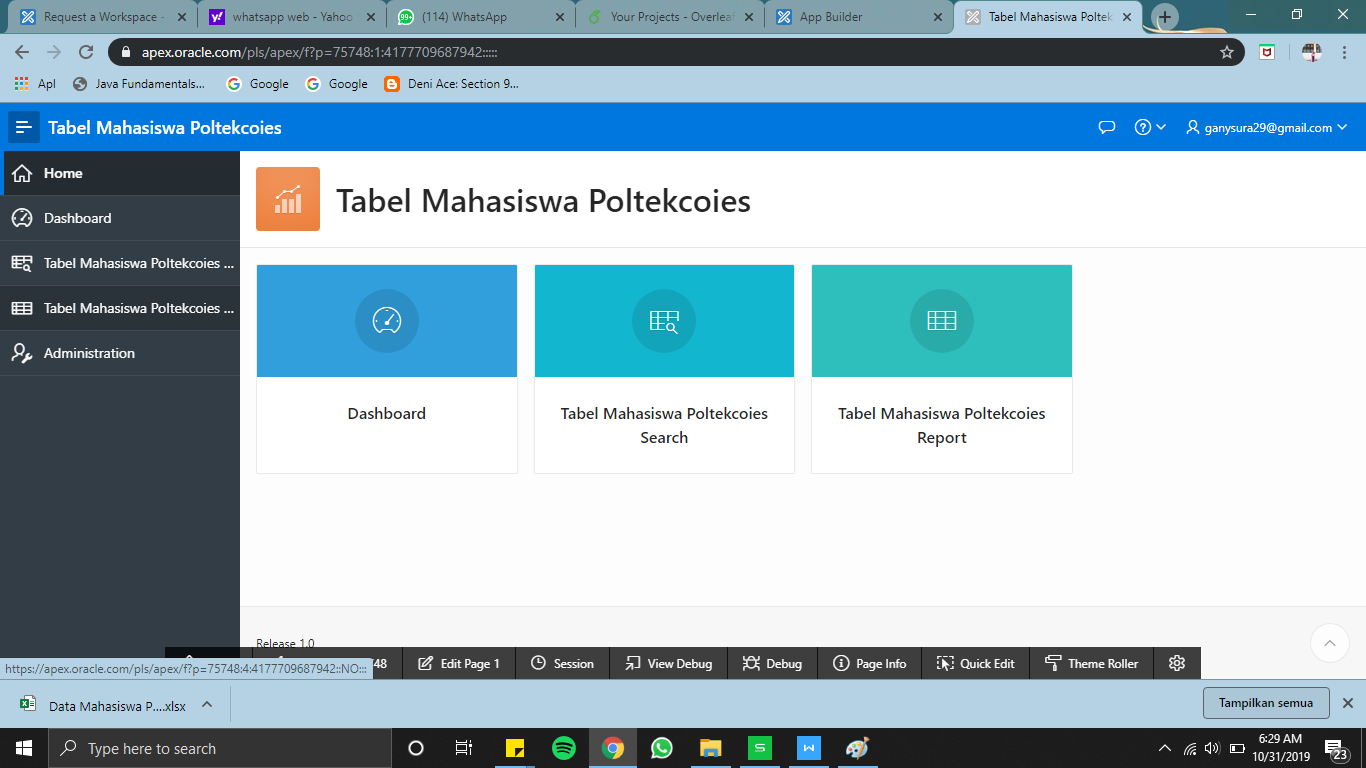
\includegraphics[width=.6\textwidth]{gambar/sebelas.png}
\end{center}
\section{setelah tabel ditampilakn , kita bisa liat pada tabel mahasiswa seacrh, pada bagan tersebut dijelaskan bahwa oracle apex ini sudah melakukan pengnormalisasian dimana sudah terpisah masing masing kriteria seperti prodi D3 Logistik sudah pisahkan dengan jurusan yang lain, hal ini jelas membuktikan bahwa aplikasi oracle apex secara otomatis mengnormalisasikan data yang di extract. }
\begin{center}
    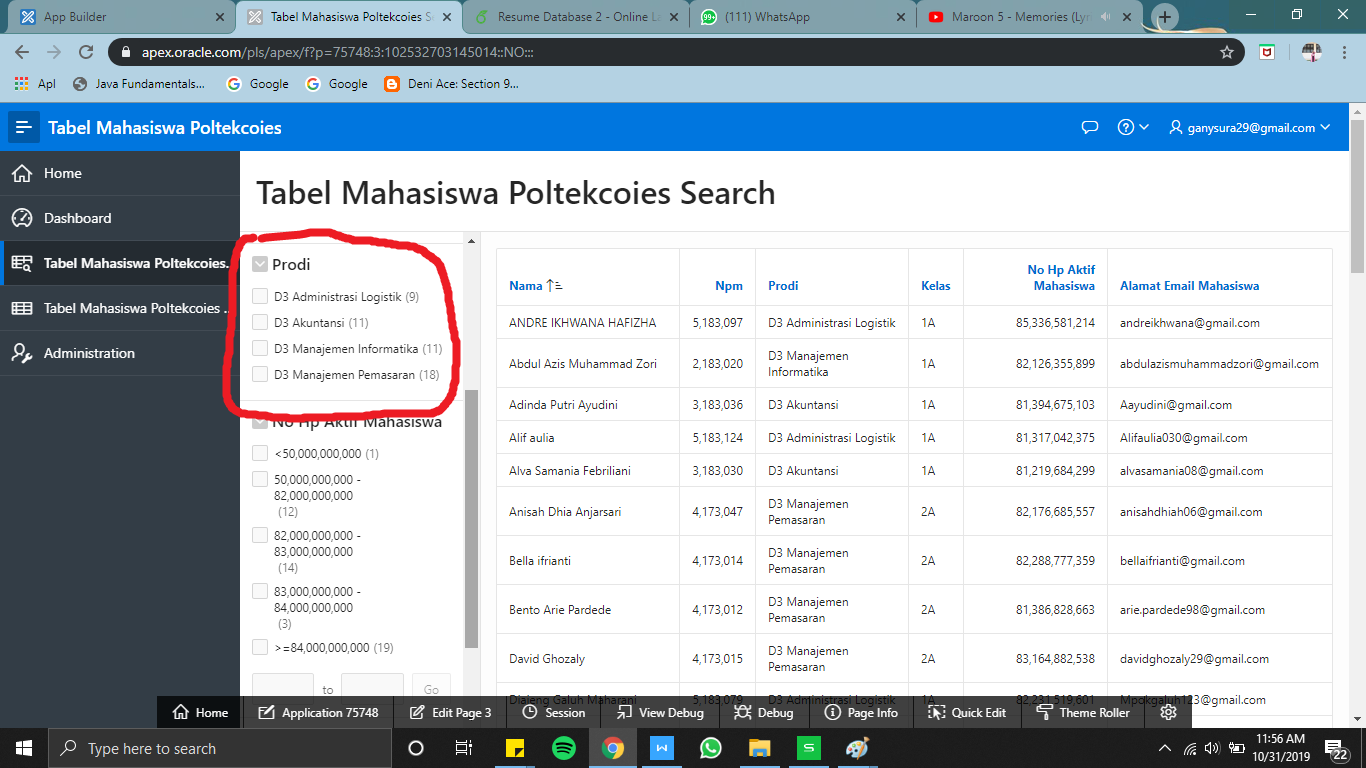
\includegraphics[width=.6\textwidth]{gambar/duabelas.png}
    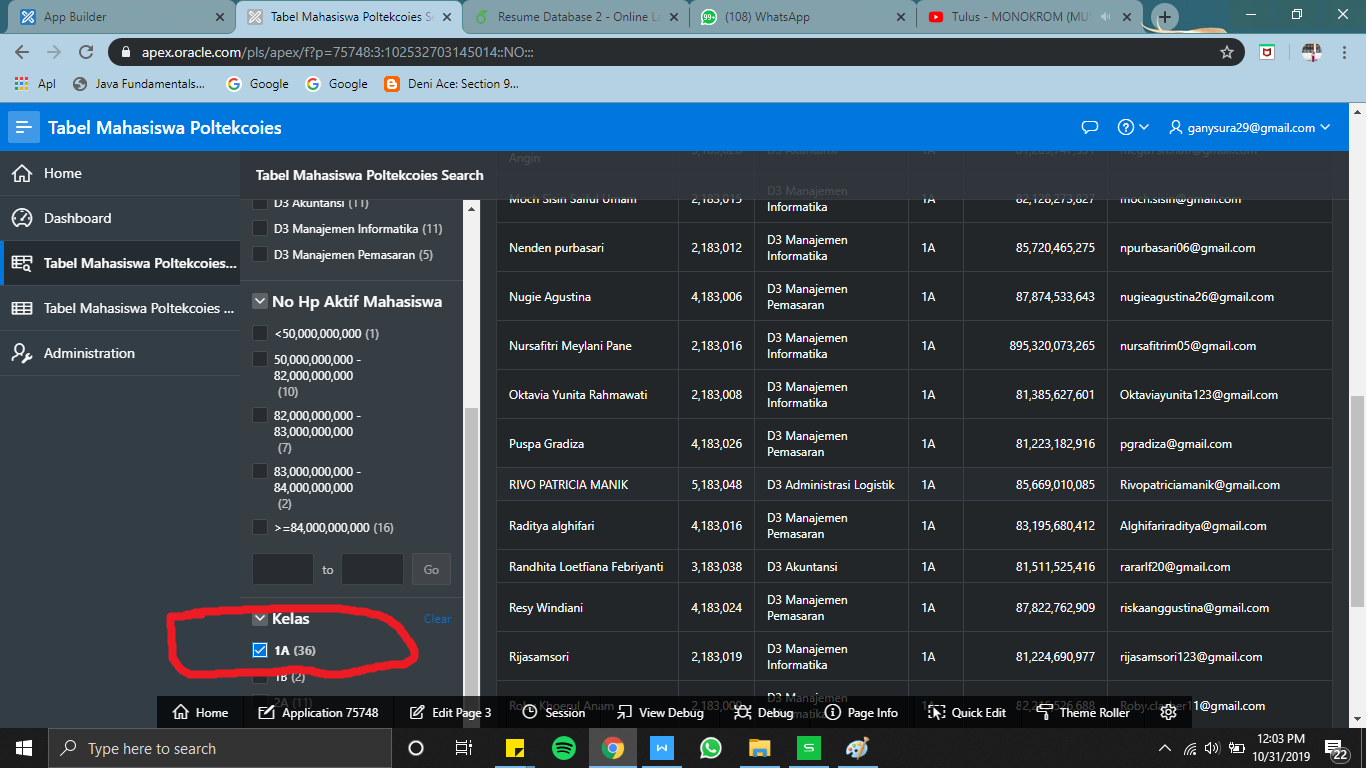
\includegraphics[width=.6\textwidth]{gambar/tigabelas.png}
\end{center}
\end{document}
